\documentclass[aspectratio=169,11pt]{beamer}
\usepackage[utf8]{inputenc}
\usepackage[T1]{fontenc}
\usepackage[spanish]{babel}
\usepackage{graphicx}
\usepackage{amsmath}
\usetheme{Madrid}
\usecolortheme{seahorse}
\setbeamertemplate{navigation symbols}{}
\title{La caída de Gwen Stacy}
\subtitle{Energía, potencia y latigazo}
\author{Diego}
\institute{Métodos Numéricos}
\date{2026}

\begin{document}

\begin{frame}
  \titlepage
\end{frame}

\begin{frame}{La pregunta}
  \begin{block}{}
    ¿Cuánta energía recibió el cuerpo y por qué no pudo liberarse gradualmente?
  \end{block}
  \begin{itemize}
    \item La energía total es finita: \(15.7\) kJ con aire, \(20.8\) kJ sin aire.
    \item Lo que mata es la \textbf{tasa}: \(P_{\max}\approx 1\) MW y
          \(a_{\max}\approx 159\) g en \(\sim 25\) ms.
    \item Escena: 42 m de caída, ancla a 43.60 m, \(x=0.40\) m.
  \end{itemize}
\end{frame}

\begin{frame}{Geometría}
  \[
    h_{\text{ancla}} - L - x = h_{\text{torso}}
  \]
  \[
    43.60 - 42.00 - 0.40 = 1.20\ \text{m}
  \]
  \begin{itemize}
    \item Masa \(m=50\) kg, \(C_dA=0.6\) m\(^2\), \(\rho=1.2\) kg/m\(^3\).
    \item Espacio libre hasta el suelo: \(1.60\) m.
    \item El ancla está en una repisa inferior, no en la cúspide de 72 m.
  \end{itemize}
\end{frame}

\begin{frame}{Modelo}
  \begin{align*}
    m\dot v &= mg - \tfrac12\rho C_dA v^2 \\
    m\ddot x &= mg - kx \\
    M_{\text{cuello}} &= m_{\text{cabeza}} r (a_t+g)
  \end{align*}
  \begin{itemize}
    \item Caída con arrastre: \(v(t)=v_t\tanh(gt/v_t)\).
    \item Resorte: \(x(t)=\frac{g}{\omega^2}(1-\cos\omega t)+\frac{v_0}{\omega}\sin\omega t\).
    \item Cuerpo anclado en el torso; cabeza y piernas como segmentos.
  \end{itemize}
\end{frame}

\begin{frame}{Solución analítica}
  \begin{columns}
    \begin{column}{0.5\textwidth}
      \begin{itemize}
        \item \(v_0=24.87\) m/s con aire; \(28.71\) m/s sin aire.
        \item \(k=195\,739\) N/m; \(x_{\max}=0.40\) m.
        \item \(a_{\max}=158.6\) g con aire; \(211\) g sin aire.
        \item \(F_{\max}=78.3\) kN; \(E=15.66\) kJ.
      \end{itemize}
    \end{column}
    \begin{column}{0.5\textwidth}
      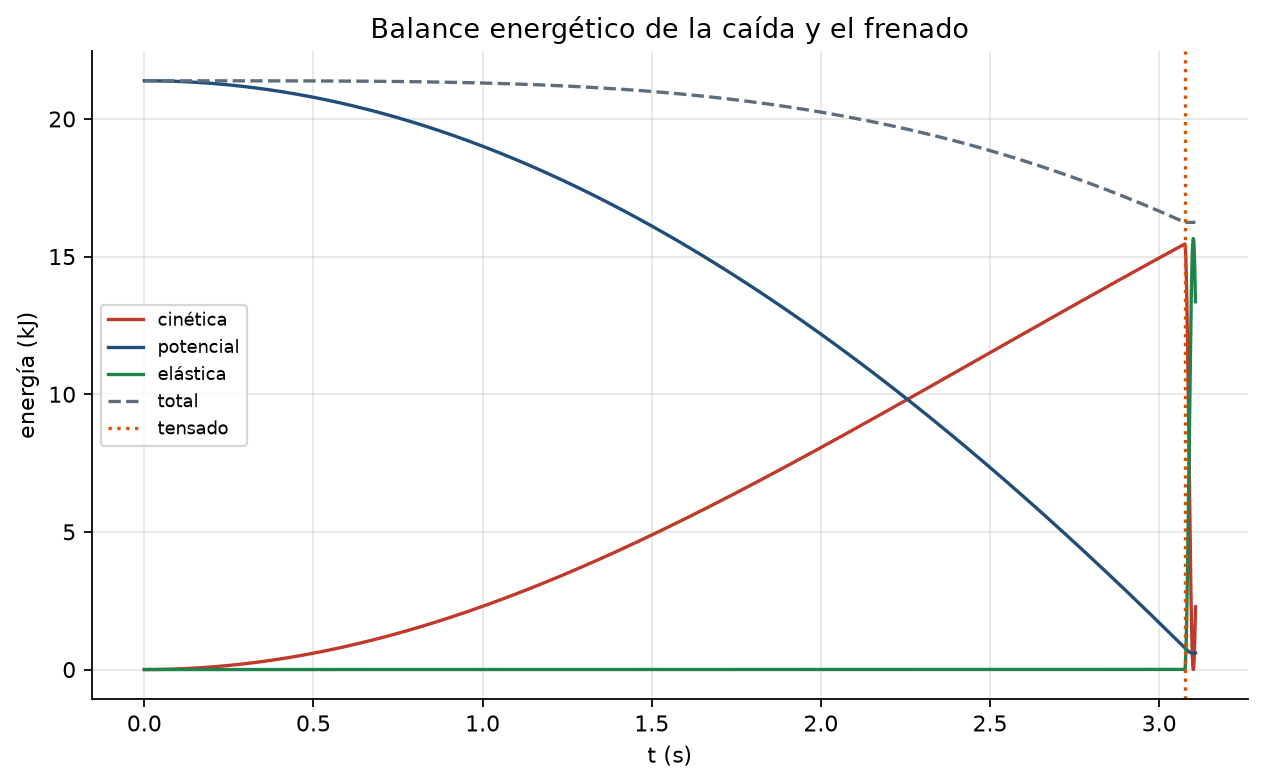
\includegraphics[width=\linewidth]{../resultados/e3_energia.png}
    \end{column}
  \end{columns}
\end{frame}

\begin{frame}{Validación Leicester (2021)}
  \begin{tabular}{lcc}
    \hline
    Magnitud & Proyecto & Paper \\
    \hline
    \(v_0\) (m/s) & 28.706 & 28.7 \\
    \(x\) (m) & 16.80 & 16.7 \\
    \(k\) (N/m) & 204.375 & 204.5 \\
    \(E\) (MPa) & 343.35 & \(\sim 343\) \\
    \hline
  \end{tabular}
  \vspace{0.5cm}
  \begin{itemize}
    \item La diferencia de \(x\) es redondeo: con 6 g exactos, \(x=0.4H\).
    \item Este test es el \emph{gate}: si no reproduce, no se avanza.
  \end{itemize}
\end{frame}

\begin{frame}{Métodos numéricos}
  \begin{itemize}
    \item Raíces: bisección, falsa posición, punto fijo, Newton, secante.
    \item EDO: Euler, Heun, Taylor 2, RK4, Euler implícito, RKF45.
    \item Integración: trapecio, Simpson, Boole, Gauss, Romberg.
    \item Lineales: LU, Thomas, Jacobi, Gauss-Seidel.
    \item Interpolación: Lagrange, Newton, spline, mínimos cuadrados.
  \end{itemize}
\end{frame}

\begin{frame}{Convergencia y rigidez}
  \begin{columns}
    \begin{column}{0.5\textwidth}
      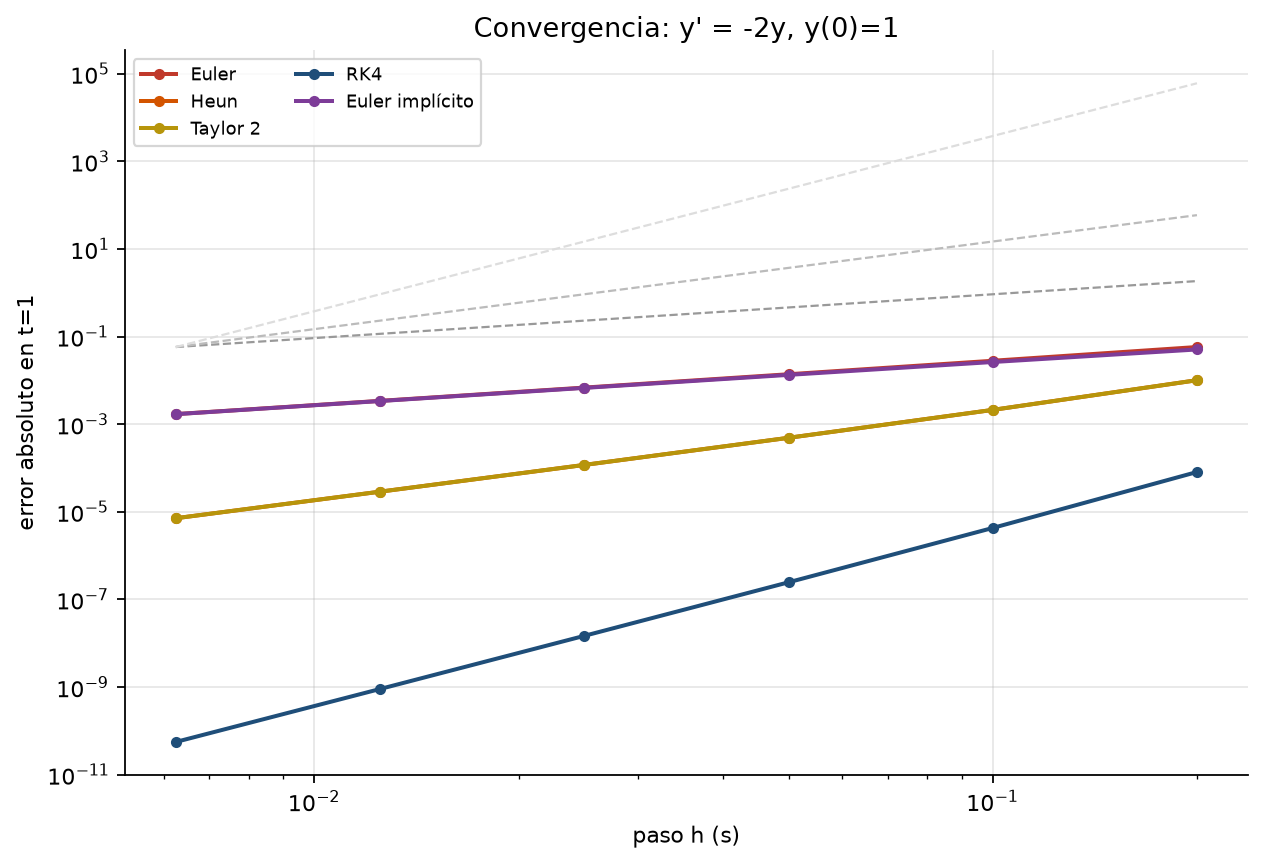
\includegraphics[width=\linewidth]{../resultados/e1_convergencia.png}
    \end{column}
    \begin{column}{0.5\textwidth}
      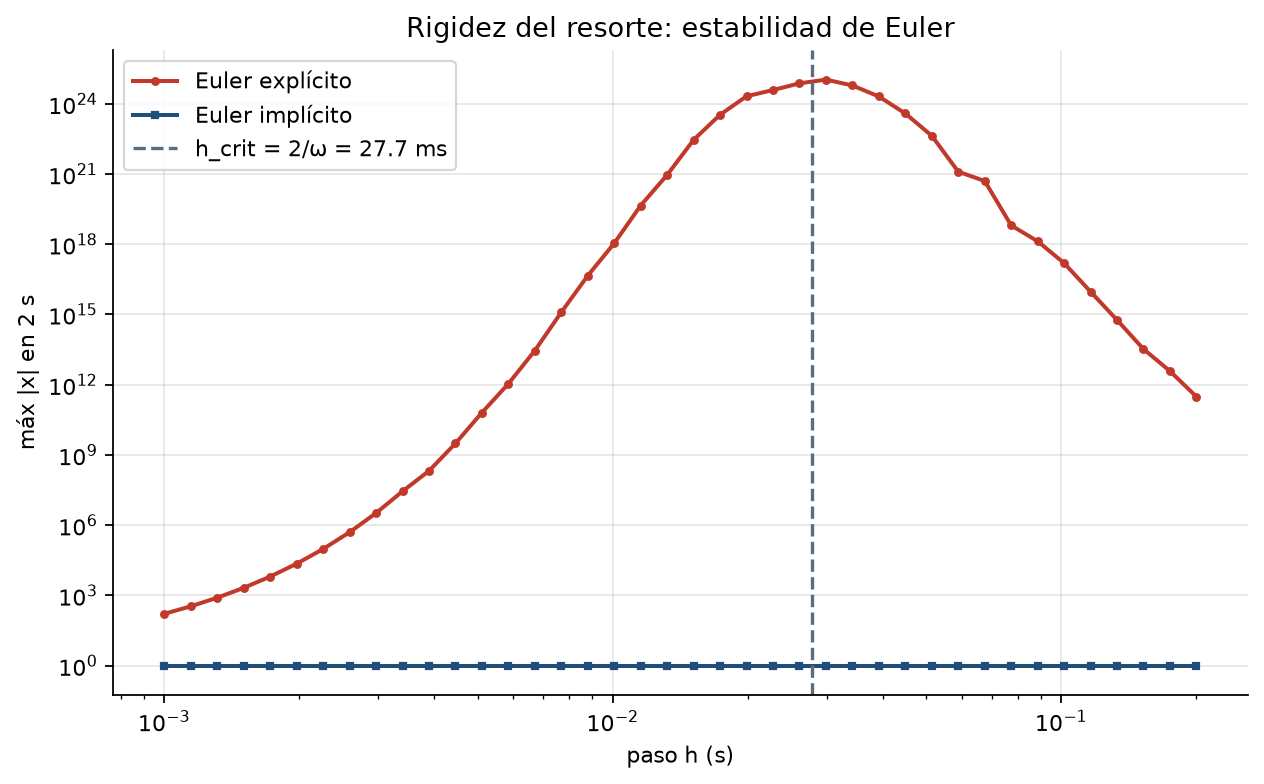
\includegraphics[width=\linewidth]{../resultados/e2_rigidez.png}
    \end{column}
  \end{columns}
  \begin{itemize}
    \item Órdenes observados: 1, 2, 4.
    \item \(h_{\text{crit}}=2/\omega=27.74\) ms.
  \end{itemize}
\end{frame}

\begin{frame}{La región factible es vacía}
  \begin{columns}
    \begin{column}{0.48\textwidth}
      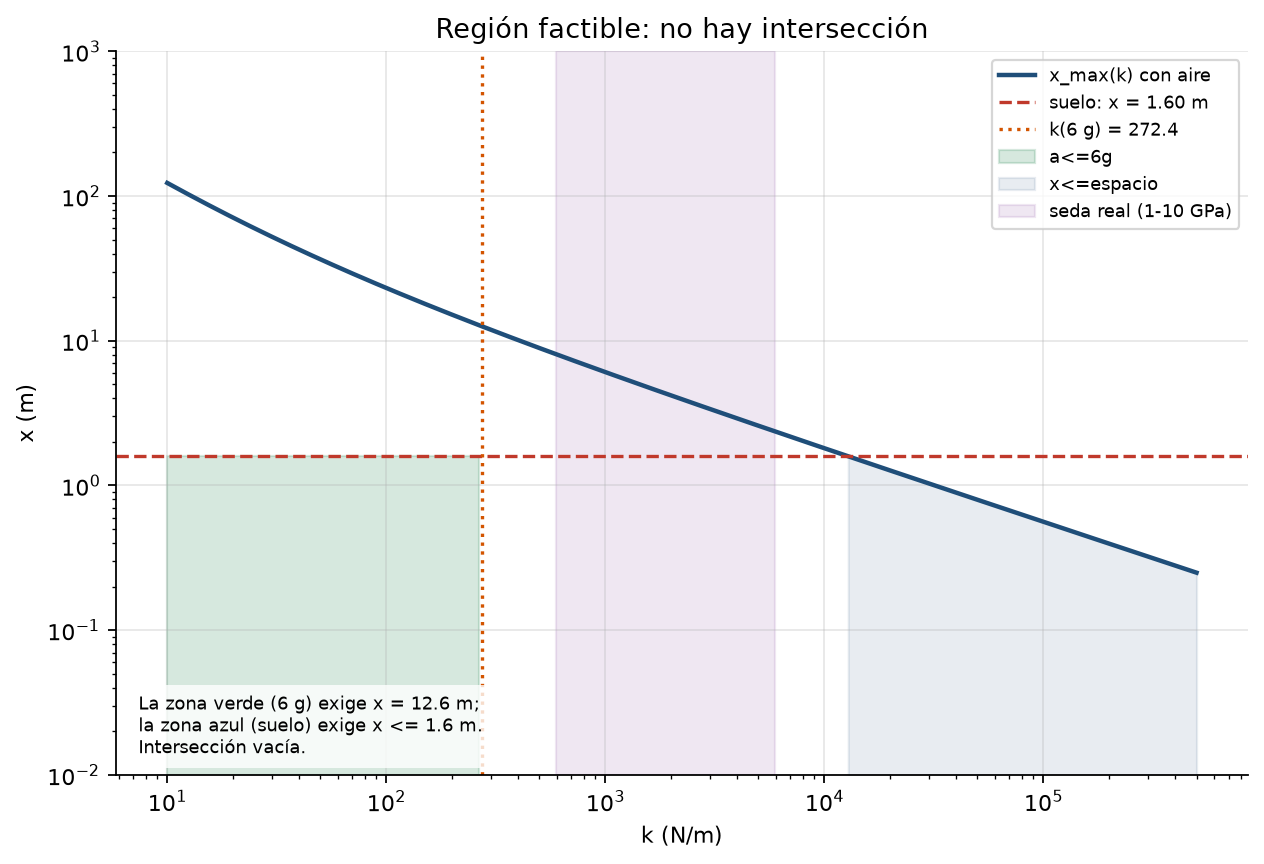
\includegraphics[width=\linewidth]{../resultados/e4_supervivencia.png}
    \end{column}
    \begin{column}{0.52\textwidth}
      \begin{itemize}
        \item 6 g: \(k=272.4\) N/m, \(x=12.61\) m, \(\varepsilon=30\%\).
        \item No tocar el suelo: \(x\le1.60\) m \(\Rightarrow E\ge21.3\) GPa,
              \(a\approx40\) g.
        \item Seda real (1--10 GPa): \(x=2.4\)--\(8.1\) m e impacto a
              \(18.6\)--\(24.9\) m/s.
        \item \textbf{No hay intersección.}
      \end{itemize}
    \end{column}
  \end{columns}
\end{frame}

\begin{frame}{Latigazo}
  \begin{columns}
    \begin{column}{0.5\textwidth}
      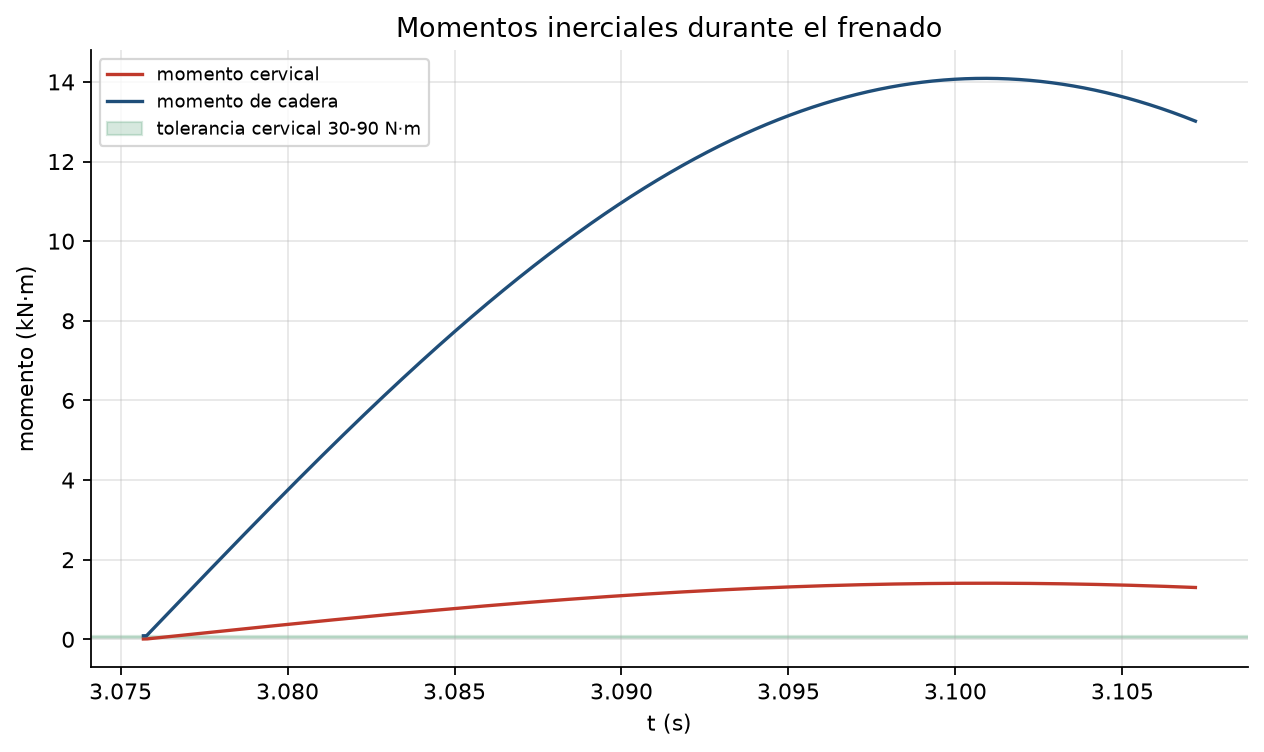
\includegraphics[width=\linewidth]{../resultados/e5_momentos.png}
    \end{column}
    \begin{column}{0.5\textwidth}
      \begin{itemize}
        \item \(M_{\text{cuello}}\approx1.41\) kN\(\cdot\)m.
        \item 20--60$\times$ el umbral de tolerancia.
        \item El torso se detiene a 1.20 m; la cabeza y las piernas no
              golpean el suelo.
      \end{itemize}
    \end{column}
  \end{columns}
\end{frame}

\begin{frame}{Monte Carlo y sensibilidad}
  \begin{columns}
    \begin{column}{0.5\textwidth}
      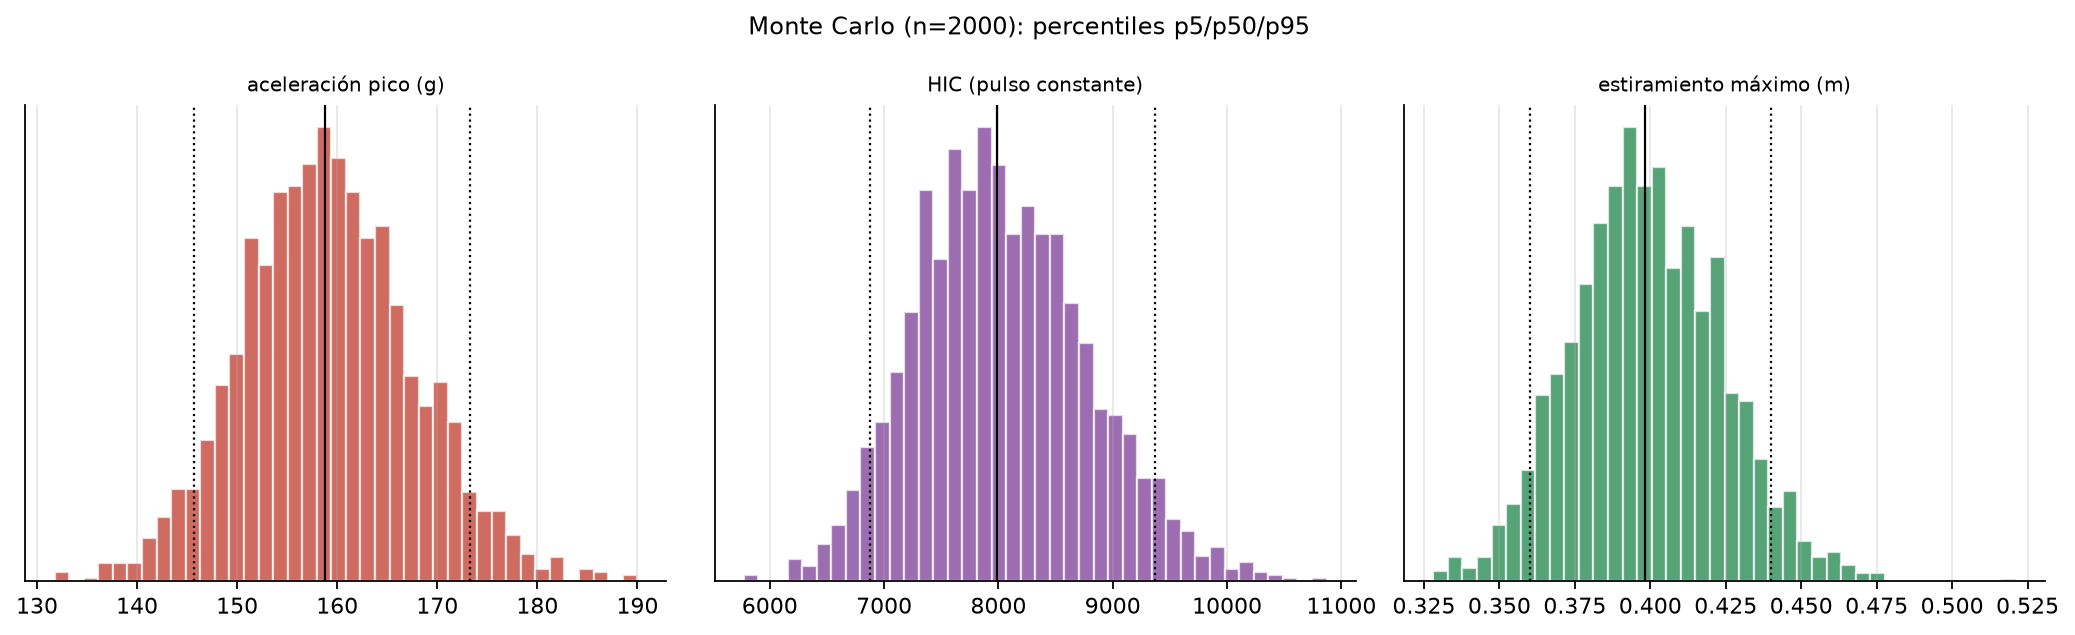
\includegraphics[width=\linewidth]{../resultados/e7_montecarlo.png}
    \end{column}
    \begin{column}{0.5\textwidth}
      \begin{itemize}
        \item \(n=2000\): 100\% con HIC \(>700\).
        \item \(a_{\max}\) p5 \(\gg 6\) g.
        \item \(k\) y la altura dominan el HIC.
      \end{itemize}
    \end{column}
  \end{columns}
\end{frame}

\begin{frame}{Interfaz}
  \begin{columns}
    \begin{column}{0.68\textwidth}
      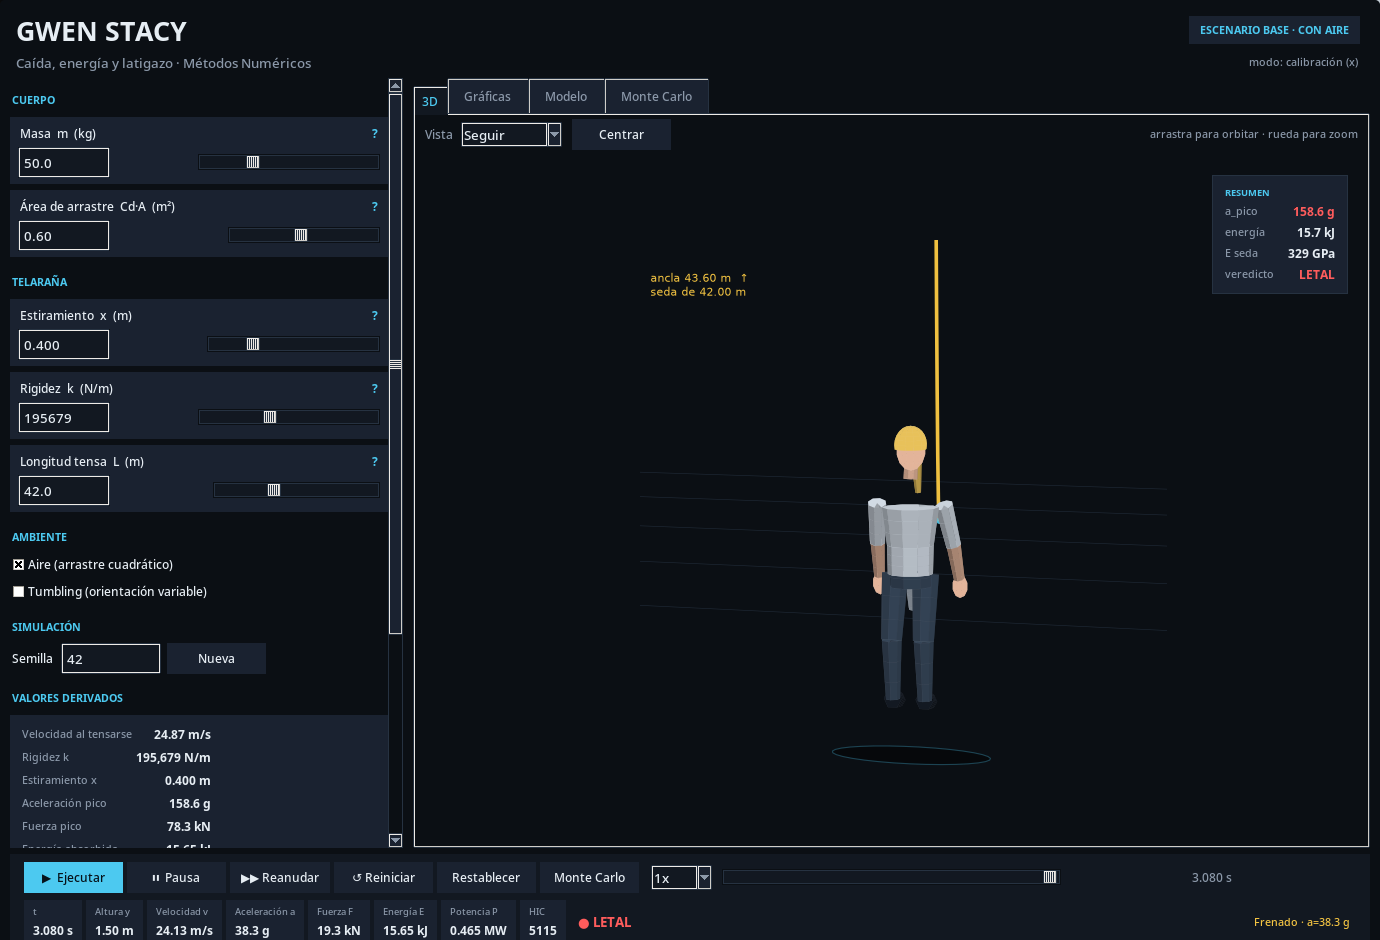
\includegraphics[width=\linewidth]{../resultados/app_captura.png}
    \end{column}
    \begin{column}{0.32\textwidth}
      \begin{itemize}
        \item Maniquí low-poly articulado.
        \item Seda unida a la cintura.
        \item Variables con unidad y tooltip.
        \item Vistas Seguir, Cuerpo y Torre.
        \item Tema oscuro pizarra + cian.
      \end{itemize}
    \end{column}
  \end{columns}
\end{frame}

\begin{frame}{Conclusiones}
  \begin{enumerate}
    \item La energía no es el problema; la potencia y la aceleración sí.
    \item Ninguna seda real cabe en 1.6 m sin impacto o sin \(\ge40\) g.
    \item El escenario de 6 g es geométricamente inviable.
    \item El latigazo cervical es el mecanismo final.
    \item El modelo reproduce Leicester y los órdenes numéricos.
  \end{enumerate}
\end{frame}

\begin{frame}{Demo}
  \begin{itemize}
    \item Ejecutar, pausar, reiniciar y recorrer la línea de tiempo.
    \item Cambiar masa, estiramiento, \(k\), longitud y semilla.
    \item Cámara lenta automática en el frenado.
    \item HUD: \(t\), \(y\), \(v\), \(a/g\), \(F\), \(E\), \(P\), HIC, semáforo.
    \item Monte Carlo en vivo.
  \end{itemize}
\end{frame}

\begin{frame}
  \centering
  \Huge Preguntas
\end{frame}

\end{document}
